\frame
{
\frametitle{\citetitle{MarcoNunoTesisLicenciatura_2002}}
\begin{columns}
    \column {0.4\textwidth}
\begin{itemize}    
\item Proyecto de asignatura de maestría: Implementación de la Pirámide en la tarjeta RC100 de Celoxica. 
\item Entrada: Video en RCA, Salida a monitor VGA.
\end{itemize}
    \column {0.3\textwidth}
\begin{center}
    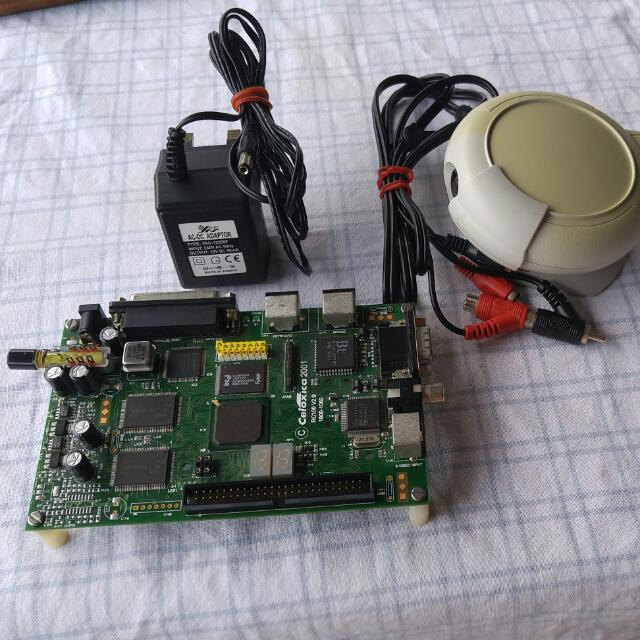
\includegraphics[width=0.9\textwidth]{Figs/celoxica_2001_rc100}
\end{center}    

    \column {0.3\textwidth} 
    \begin{center}
    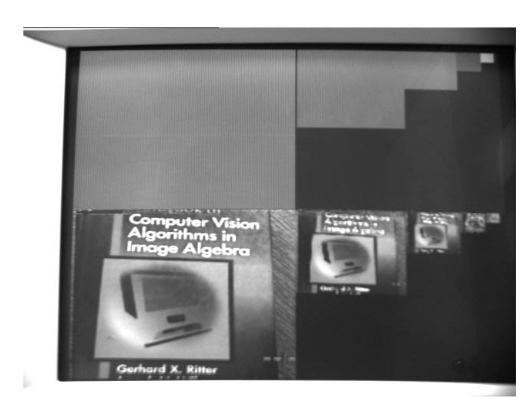
\includegraphics[width=0.9\textwidth]{Figs/2002_PiramideMonitor_RC100}\\
        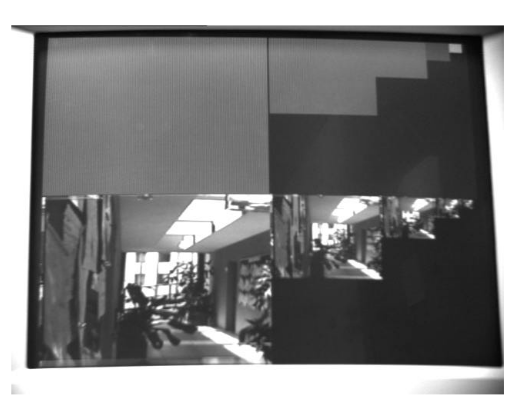
\includegraphics[width=0.9\textwidth]{Figs/2002_PiramideMonitor_RC100_2}
            \end{center}
\end{columns}     

\footnotetext[1]{\fullcite{MarcoNunoTesisLicenciatura_2002}}
}

\frame{
\frametitle{Arquitectura Propuesta}
\begin{columns}
    \column {0.5\textwidth}
 \begin{itemize} 
\item Procesamiento de video en tiempo real.
\item Procesamiento simultaneo (doble búffer): Un proceso almacenaba un frame de memoria, mientras que otro procesaba el frame previamente almacenado.
\item Lenguaje: Handel-C (RIP).
\item DK1 Design Suite.
\item FPGA: Spartan-II.
\item Tarjeta: RC-100 de Celoxica.
    
\end{itemize}
    
    \column {0.5\textwidth} 
    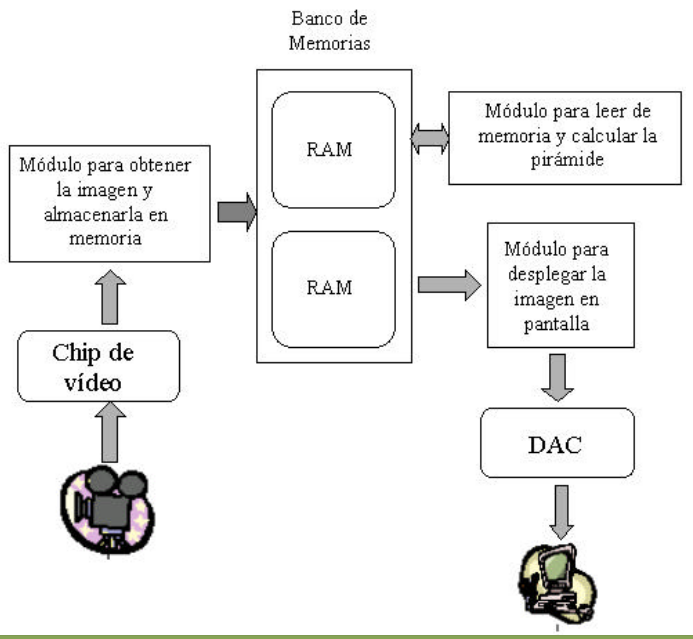
\includegraphics[width=0.9\textwidth]{Figs/2002_PiramideMonitor_RC100_Arquitectura_3}
\end{columns}     
}

